\section{Comparing the results of the second journey}

This section makes another comparison between the three approaches. The path through the application is shown in figure \ref{fig:results:evaluation-second-path}.


\ifshowImages
\begin{figure}[H]
\centering
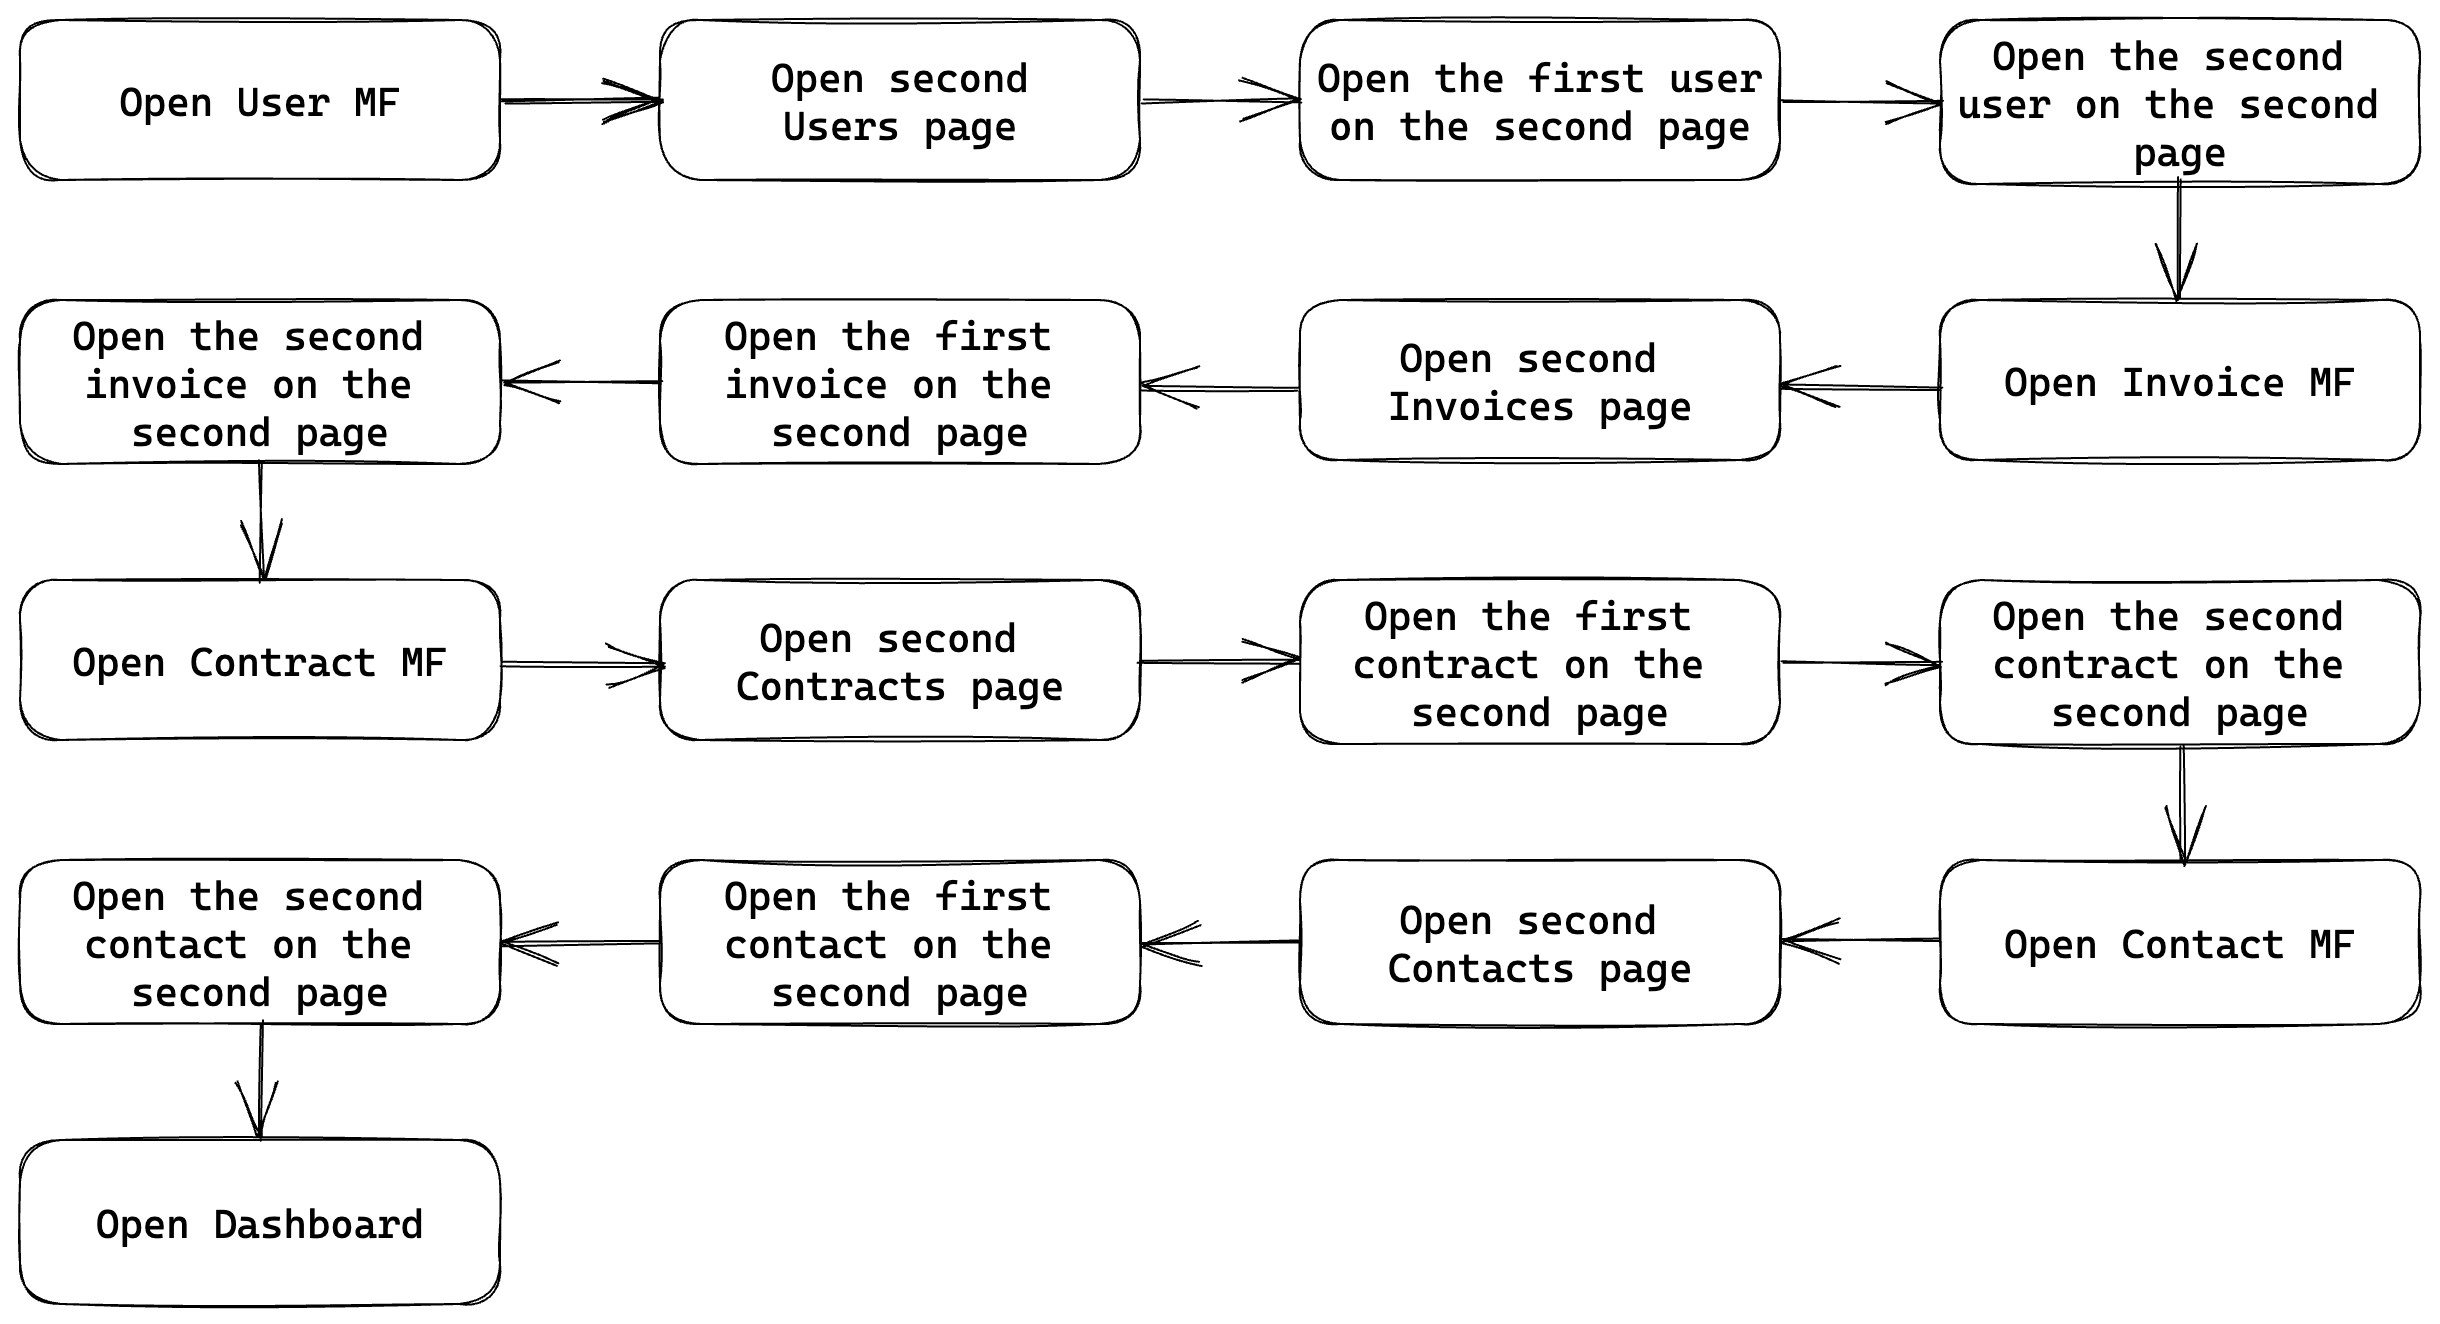
\includegraphics[width=1\linewidth]{images/results/evaluation-second-path.png}
\caption{The second user journey through the application to measure the performance of the micro-frontend architecture.}\label{fig:results:evaluation-second-path}
\end{figure}
\fi

\noindent For this path through the application \textbf{59} queries in total have to be executed against the
GraphQL \ac{API}, when no caching mechanism are implemented.

\begin{table}[H]
    \begin{tabular}{|l|l|l|l|}
    \hline
                                    & Request Size (B) & Response Size (B) & Request Amount  \\
    \hline
     No Reduction, Shared Cache     &  16884       &  8364416   & 37 \\
     \hline
     Reduction, Shared Cache        &  14718       &  8361306   & 37 \\
     \hline
     \hline
    \textbf{Diff}                   & \textbf{2166} & \textbf{3110} & \textbf{11} \\
    \hline
    \textbf{Reduction (\%)} & \textbf{11\%} & \textbf{0\%} & \textbf{-} \\
     \hline
    \end{tabular}
    \caption{Comparing the requests and responses of the first- and second-approach.}
    \label{tab:serious-game-comparison}
\end{table}

\begin{table}[H]
    \begin{tabular}{|l|l|l|l|}
    \hline
                                    & Request Size (B) & Response Size (B) & Request Amount  \\
    \hline
     No Reduction, No Shared Cache     &  22955        &  10713304   & 62 \\
     \hline
     Reduction, Shared Cache        &  14718        &  8361306   & 37 \\
     \hline
     \hline
    \textbf{Diff}                   & \textbf{8237} & \textbf{2351998} & \textbf{25} \\
    \hline
    \textbf{Reduction (\%)} & \textbf{11\%} & \textbf{0\%} & \textbf{-} \\
     \hline
    \end{tabular}
    \caption{Comparing the requests and responses of the first- and third-approach.}
    \label{tab:serious-game-comparison}
\end{table}

\begin{table}[H]
    \begin{tabular}{|l|l|l|l|}
    \hline
                                    & Request Size (B) & Response Size (B) & Request Amount  \\
    \hline
     No Reduction, No Shared Cache     &  22955        &  10713304   & 62 \\
     \hline
     No Reduction, Shared Cache        &  16884        &  8364416   & 37 \\
     \hline
     \hline
    \textbf{Diff}                   & \textbf{6071} & \textbf{2348888} & \textbf{25} \\
    \hline
    \textbf{Reduction (\%)} & \textbf{11\%} & \textbf{0\%} & \textbf{-} \\
     \hline
    \end{tabular}
    \caption{Comparing the requests and responses of the second- and third-approach.}
    \label{tab:serious-game-comparison}
\end{table}
